\documentclass{article}
\usepackage{multicol}
\usepackage{graphicx}% Include figure files
\usepackage{dcolumn}% Align table columns on decimal point
\usepackage{bm}% bold math
\usepackage{hyperref}% add hypertext capabilities
\usepackage{booktabs}
\usepackage{listings}
\usepackage{mathtools}
\usepackage{amsmath}
\renewcommand{\abstractname}{\vspace{-\baselineskip}}
\bibliographystyle{plain}
\usepackage[utf8]{inputenc}
\usepackage{verbatim} %for aa inkludere filer med tegn LaTeX ikke liker
\usepackage{mathpazo}
\usepackage{float}
\usepackage{algpseudocode}
\newcommand\numberthis{\addtocounter{equation}{1}\tag{\theequation}}
\usepackage[left=20mm,right=20mm,top=33.95mm,bottom=33.95mm]{geometry} 
% Justerer bredden på columns.
\setlength{\columnsep}{1cm}

\begin{document}

\title{Solving the heat equation numerically and simulating the Fennoscandian lithosphere}
\author{Sebastian Amundsen, Marcus Berget and Andreas Wetzel}

\maketitle

\begin{abstract}

We found that the heat equation can be solved using the explicit forward method, the implicit backward Euler method and the Crank- Nicholson scheme. The stability condition of the explicit method is decided by the $\Delta t \leq \Delta x^2/2$. We found that the implicit methods were stable regardless of this condition. The Forward Euler method was the fastest numerical solver, being 76\% and 75 \% faster than Crank Nicholson and Backward Euler respectively. We successfully used the forward Euler method to solve the two-dimensional heat equation. We simulated a simplified model of the Fennoscandian lithosphere for 10 Gy, starting 2 Gy ago. At the bottom of the lithosphere we assumed a temperature of $T=1300\text{C}^{\circ}$ which caused a linear temperature distribution up to the surface where we assumed a temperature of $T=8\text{C}^{\circ}$. The enrichment of radioactive elements in the lithosphere will cause a temperature increase across the whole lithosphere, with the most dramatic temperature increase in the middle of the lithosphere.
\end{abstract}

\begin{multicols}{2}

\section{Introduction}


Most partial differential equations, or PDE's, can seldom be solved analytically, which is where numerical methods for solving them comes in very handy. It is therefore very important to understand the pros and cons of different methods of solving PDE's numerically. 
In this project we test three algorithms for solving such PDE's using finite difference schemes. \\ We specifically want to solve the heat equation in one dimension using three different methods, namely the forward Euler method, the backward Euler method and the Crank-Nicholson scheme. We then compare our numerical results to the analytical solution. The comparison is done by calculating the root mean square error and by looking at the deviation between numerical and analytical values for each of the algorithms. We will also be testing the stability conditions of the solvers. We then expand the most suited numerical method for solving the heat equation to two dimensions. \\ 
Finally, we will showcase how the most suitable of these methods can be implemented numerically to solve a physical problem. This is done by developing a model for the Fennoscandian lithosphere, and simulating the time evolution of it's temperature distribution. 

\section{Theory}

\subsection{Heat equation}

The general heat equation can be written as,
\begin{equation}
	\frac{\partial T(\textbf{x}, t)}{\partial t} = \frac{k}{C\rho}\nabla^2 T(\textbf{x}, t). \label{eq:gen_heat}
\end{equation}
where $\textbf{x}$ is the spatial vector, $t$ is time, $c_p$ is the specific heat capacity, $\rho$ is the density and $k$ is the thermal conductivity. We can then gather all the constants in the diffusion constant, $D=\frac{k}{C\rho}$. For the first part of the project we will just set the diffusion constant equal to one. The heat equation in one dimension then becomes, 
\begin{equation}
	\frac{\partial T(x,t)}{\partial t} = \frac{\partial^2 T(x,t)}{\partial x^2}, \label{eq:heat_one}
\end{equation}
or 
\begin{equation}
	T_{xx}=T_t.
\end{equation}
\subsection{Numerical methods for solving the heat equation}
We set the initial conditions of equation \eqref{eq:heat_one} at $t=0$ to,
\begin{align}
	T(x,0)=0, \quad 0<x<L
\end{align}
where $L=1$ is the length of the x-region of interest. We set the boundary conditions to
\begin{align}
	T(0, t)=0, \quad t\geq 0,
\end{align}
and
\begin{align}
	T(L, t)= 1, \quad t\geq 0.
\end{align}
Equation \eqref{eq:heat_one} with the mentioned initial conditions and boundary conditions can be solved numerically using the forward Euler method, the backward Euler method and the implicit Crank-Nicholson scheme. 

\subsubsection{Explicit forward Euler method}
We proceed with equation \eqref{eq:heat_one} and the mentioned initial/boundary conditions. We define the step length for the spatial variable $x$,
\begin{equation}
	\Delta x=\frac{1}{n+1}.
\end{equation}
The position after i steps and time after j steps are then given by,
\begin{align*}
	t_j &= j\Delta t, \quad j \geq 0, \\
	x_i &= i\Delta x, \quad 0 \leq i \leq n+1.
\end{align*}
By using the forward formula to approximate the derivatives we obtain 
\begin{comment}
\begin{equation}
	T_t = \frac{T(x_i, t_j+\Delta t)-T(x_i, t_j)}{\Delta t}
\end{equation}
and 
\begin{equation}
	T_{xx}= \frac{T(x_i+\Delta x , t_j)-2T(x_i, t_j)+T(x_i-\Delta x, t_j)}{{\Delta x}^2}
\end{equation}
\end{comment}

\begin{equation}
	T_t=\frac{T_{i,j+1}-T_{i,j}}{\Delta t}
\end{equation}
and
\begin{equation}
	T_{xx}=\frac{T_{i+1,j}-2T_{i,j}+ T_{i-1,j}}{{\Delta x}^2}.
\end{equation}
Defining the value $\alpha = \Delta t/ {\Delta x}^2 $, the one-dimensional heat equation can be rewritten as
\begin{equation}
	T_{i,j+1}=\alpha T_{i-1,j}+(1-2\alpha )T_{i,j} + \alpha T_{i+1, j}. \label{for_eul}
\end{equation}
We can then see than since the initial conditions are known, one could use equation \eqref{for_eul} to find the temperature in the next time step, which one could use to the find the temperature after two time steps, and so on. This algorithm is an explicit scheme, since the temperature in the next time step is explicitly given. 

\subsubsection{Implicit backward Euler method}

Here, we do just as for the forward Euler method, but instead of using the forward formula to approximate the first derivative, we use the backward formula,
\begin{equation}
T_t=\frac{T_{i,j}-T_{i,j-1}}{\Delta t}.
\end{equation}
The spatial second derivative becomes just as for the explicit scheme, 
\begin{equation}
T_{xx}=\frac{T_{i+1,j}-2T_{i,j}+ T_{i-1,j}}{{\Delta x}^2}.
\end{equation}
Again, by defining $\alpha = \Delta t/ {\Delta x}^2$ we obtain
\begin{equation}
T_{i,j-1}=-\alpha T_{i-1,j}+(1+2\alpha )T_{i,j} - \alpha T_{i+1, j}. \label{eq:back_eul}
\end{equation}

The only unknown quantity in equation \ref{eq:back_eul} is $T_{i,j-1}$, we can then define the matrix A,

\begin{equation}
A = 
\begin{bmatrix}
1+2\alpha & -\alpha & 0 & \cdots & 0 \\
-\alpha & 1+2\alpha & -\alpha & \cdots & 0  \\
\vdots  & \ddots  & \ddots & \ddots & \vdots  \\
\vdots  & \vdots  & \ddots & \ddots & -\alpha  \\
0 & 0 & \cdots & -\alpha & 1+2\alpha
\end{bmatrix}
\end{equation}

so that we can reformulate the problem as a matrix vector multiplication equation:

\begin{equation}
A V_j=V_{j-1}
\end{equation}

We can then write the problem as:

\begin{equation}
\begin{split}
V_j &= A^{-1}V_{j-1}=A^{-1}(A^{-1}V_{j-2})\\
&=A^{-1}(A^{-1}(A^{-1}V_{j-3}))=A^{-j}V_0
\end{split}
\end{equation}
we can then use the tridiagonal algorithm discussed in Appendix B.1 to solve this set of linear equations for every time step. 

\subsubsection{Crank-Nicholson scheme}

The Crank-Nicholson scheme a bit more tedious to derive, so we will go ahead just give the approximations it uses for the time and spatial derivative:
\begin{equation}
T_t = \frac{T(x_i,t_j+\Delta t)-T(x_i,t_j)}{\Delta t}
\label{eq:T_t}
\end{equation}
and 
\begin{equation}
\begin{split}
&T_{xx}=\frac{1}{2}\bigg( \frac{T(x_i+\Delta x, t_j)-2T(x_i,t_j)+T(x_i-\Delta x, t_j)+}{{\Delta x}^2} \\
&\frac{T(x_i + \Delta x, t_j + \Delta t )-2T(x_i,t_j+\Delta t)+T(x_i -\Delta x, t_j + \Delta t)}{{\Delta x}^2}\bigg)
\label{eq:T_xx}
\end{split}
\end{equation}

We then combine equation \ref{eq:T_t} and \ref{eq:T_xx}, where the left side is given by $t_j+\Delta t$ and the right by $t_j$:

\begin{equation}
\begin{split}
&-\alpha T(x_i-\Delta x, t_j+\Delta t)+(2+2\alpha) T(x_i, t_j+\Delta t)\\
&-\alpha T(x_i+\Delta x,t_j+\Delta t)=\alpha T(x_i-\Delta x, t_j)+(2-2\alpha)T(x_i,t_j)\\
&+\alpha T(x_i+\Delta x, t_j)
\end{split}
\end{equation}

Where we have used that $\alpha = \frac{D\Delta t}{\Delta x^2}$. We can write this as a tridiagonal matrix system:

\begin{equation}
(2I+\alpha B)V_j=(2I-\alpha B)V_{j-1}
\label{eq:IB}
\end{equation}

We can rewrite equation \ref{eq:IB} as:

\begin{equation}
V_j = (2I+\alpha B)^{-1}(2I-\alpha B)V_{j-1}
\end{equation}

Where I is the identity matrix and B is given by:

\begin{equation*}
B = 
\begin{bmatrix}
2 & -1 & 0 & \cdots & 0 \\
-1 & 2 & -1 & \cdots & 0  \\
\vdots  & \ddots  & \ddots & \ddots & \vdots  \\
\vdots  & \vdots  & \ddots & \ddots & -1  \\
0 & 0 & \cdots & -1 & 2
\end{bmatrix}
\end{equation*}

The truncation error for the Crank Nicholson scheme goes as $O(\Delta t^2)$ and is stable for all combinations of $\Delta x$ and $\Delta y$. 

\subsection{Analytical solution for one dimensional heat equation}

It is beneficial to have a analytical solution which we can compare our numerical methods to. For the one dimensional diffusion equation we have the analytical expression:

\begin{equation}
\begin{split}
&u(x,t)=x/L+\\
&\sum_{n=1}^{\infty}\frac{2(\pi n \cos{(\pi n)}-\sin{(\pi n)})}{\pi^2n^2}\sin{(n\pi x/L)}e^{-n^2\pi^2t/L}
\end{split}
\label{eq:ana_sol}
\end{equation}

Where g(x) is a function of position. The calculations are given in appendix B. 

\subsection{Heating of the Fennoscandian lithosphere}
The lithosphere is the solid upper-most part of the earth, consisting of the mantle, lower crust and upper crust. We will focus on an area of the earth's lithosphere located in Scandinavia, which we will call the fennoscandian lithosphere. About 1 Gy ago the oceanic lithosphere on the west coast of Norway was subducted under the fennoscandian lithosphere. This process released radioactive elements trapped in, and heating, the fennoscandian lithosphere. 

\subsubsection{Parameters of the model}
The boundary conditions are 8 $\text{C}^{\circ}$ at the surface and 1300 $\text{C}^{\circ}$ at the bottom at a depth of 120 km. We will assume a constant density of $\rho=3500 \, \text{kg/m}^3$, a constant thermal conductivity of $\kappa=2.5 \text{W/m/} \text{C}^{\circ}$ and a constant specific heat capacity of $c_p=1000 \text{J/kg/}\text{C}^{\circ}$. Before the subduction of the oceanic lithosphere we will assume that the fennoscandic lithosphere already contained radioactive elements causing the following heat production:
\[
P(z, t) =
\begin{cases}
1.4 \, \mu \text{W/m}^3 &  0 \, \text{km} < z < 20 \, \text{km} \\
0.35 \, \mu \text{W/m}^3 &  20 \, \text{km} < z < 40 \, \text{km} \\
0.05 \, \mu \text{W/m}^3 &  z > 40 \, \text{km} \\
\end{cases}
\]
for $t\in [0, 1]$ Gy. We will assume that the additional heat production caused by the enrichment of radioactive elements at 1 Gy is $\text{P}_0=0.5 \, \mu \text{W/m}^3$. We assume that this additional heat is produced is at 40$\%$ by U, 40$\%$ by Th, and 20$\%$ by K, which have halflives of 4.47 Gy, 14.0 Gy, 1.25 Gy respectively. The reduction of radioactive sources over time will cause the additional heat production to decrease as function of time, which can be described as follows:
\begin{equation}
	P_R(t) = P_0\Bigg(0.4\bigg(\frac{1}{2}\bigg)^{t/4.47}+0.4\bigg(\frac{1}{2}\bigg)^{t/14.0}+0.2\bigg(\frac{1}{2}\bigg)^{t/1.25}\Bigg)
\end{equation}


\section{Method}

\subsection{One dimensional model}

We start by implementing our numerical methods in one dimension. We begin by initializing our boundary and initial conditions. We will be testing our algorithms with different spatial steps given $\Delta x =1/10$ and $\Delta x = 1/100$, where $\Delta t$ will be dictated by the stability limit of the explicit scheme. This limit is given $\alpha<0.5$. We therefore need to adjust the duration of each time step and the number of time steps we are using to fulfill this explicit limit. We wish to study the algorithms during two different occasions. There will be an equilibrium time before our solution becomes stable. It is relevant to study the system during this equilibrium time $t_1$ and when the system is close to stationary $t_2$. This will be done for each spatial step $\Delta x$. The truncation error should go according to Table \ref{tab:a}.

\subsubsection{Comparison between numerical and analytical model}

We can test the stability and precision of our numerical algorithms by comparing our numerical approximations to our analytical solution given equation \ref{eq:ana_sol}. We need to set N to something less than $\infty$ due to numerical limitations. We set N=1000. We compare our numerical and analytical results both visually by using plots and by studying the relative root mean square error (RRMSE). This will give us insight to how well our numerical approximations represent the one dimensional heat equation. We can then choose which of the three methods (Forward Euler, Backward Euler and Crank-Nicholson) best fit our analytical solution. The relative root mean square error is given by:

\begin{equation}
RRMSE = \sqrt{\frac{\frac{1}{n}\sum_{i=1}^n(u_{ana}-u_{num})^2}{\sum_{i=1}^n u_{ana}^2}}
\end{equation}

Where $u_{ana}$ is the analytical solution and $u_{num}$ is the numerical approximation \cite{97}. We will also be plotting the difference between the analytical solution and the values given the algorithms. This is to be done for both $\alpha>0.5$ and $\alpha<0.5$, which hopefully will showcase the stability of the implicit methods. To obtain the different values for $\alpha$ we adjust the duration of each time step in our simulation. The boundary given time steps $\Delta t$ and spatial steps $\Delta x$ for the explicit method is:

\begin{equation}
\Delta t \leq \Delta x^2/2
\end{equation}

We wish to study the case where this boundary is fulfilled and when it is unsatisfied. 

\subsection{Extending to two dimensions}

We still assume dimensionless quantities and set the diffusion constant $D=1$, just as for the one dimensional case. The two dimensional heat equation then becomes,
\begin{equation}
\frac{\partial T}{\partial t} = \bigg( \frac{\partial^2 T}{\partial x^2} + \frac{\partial^2 T}{\partial y^2} \bigg)
\end{equation}
By assuming a square lattice of length $L$ with an equal amount of points in the x-direction as in the y-direction we are ready to discretize the time and spatial derivatives. We get,
\begin{equation}
T_{xx} \approx \frac{T^l_{i+1, j}-2T^l_{i,j}+T^l_{i-1,j}}{h^2}
\end{equation}
where $h= \frac{L}{n+1}=\Delta x = \Delta y$. The second derivative of $y$ reads
\begin{equation}
T_{yy} \approx \frac{T^l_{i, j+1}-2T^l_{i,j}+T^l_{i,j-1}}{h^2}
\end{equation}
By using the forward Euler method we find the following equation for the first derivative of time 
\begin{equation}
T_t\approx \frac{T^{l+1}_ {i,j}-T^l_{i,j}}{\Delta t}.
\end{equation}
Combining the three equations above we finally get an explicit expression for the temperature after $\Delta t$
\begin{equation}
T^{l+1}_{i,j}=T_{i,j}^l+\alpha(T_{i+1,j}^l+T_{i-1,j}^l+T_{i,j+1}^l+T_{i,j-1}^l-4T_{i,j}^l)
\end{equation}
where $\alpha = \Delta t/ h^2$ and the stability condition of $\alpha\leq 0.5$ still holds. We set the all the boundaries of the square lattice to $T=0.0$, while every other point in the lattice has $T=1.0$. We set the length to $L=10$, using a $100 \times 100$ square lattice. We set $\Delta t = 1\times 10^{-5}$ and let the simulation run for $5\times10^4$ time steps. 

\subsection{Heating of the Fennoscandian lithosphere}

We will assume that the fennoscandian lithosphere will be affected equally across the whole area surface, so that the depth is the only spatial dimension affecting the time evolution of the temperature. We also have to take in to account the heat production caused by radioactive elements. This translates to the heat equation as:
\begin{equation}
	\frac{\partial T}{\partial t}= \frac{P}{\rho c_p} + \frac{\kappa}{\rho c_p}\frac{\partial^2 T}{\partial^2 z}
\end{equation}
where z is the depth. We define $z=0$ as the surface, so that the depth direction is down in to the lithosphere. We set $D=\frac{\kappa}{\rho c_p}$ and introduce $z=a\hat{z}$, so that the heat equation becomes
\begin{equation}
	\frac{\partial T}{\partial t}=\frac{P}{\rho c_p}+\frac{1}{D a^2}\frac{\partial^2 T}{\partial^2 \hat{z}}.
\end{equation}
We then choose $Da^2=1$ so that the final heat equation becomes,
\begin{equation}
	\frac{\partial T}{\partial t}=\frac{P}{\rho c_p}+\frac{\partial^2 T}{\partial^2 \hat{z}}.
\end{equation}
By using the exact same approximations as for the forward Euler method, we have an explicit expression for temperature after in the next time step:
\begin{equation}
	T_{i,j+1}= \frac{P}{\rho c_p}\Delta t + \alpha T_{i-1,j}+(1-2\alpha )T_{i,j} + \alpha T_{i+1, j}
\end{equation}
where $\alpha=\frac{\Delta t}{\Delta x ^2}$ . 
When initializing the temperature we will consider the state without radioactive elements, but in thermal equilibrium. The temperature distribution must therefore be linear:
\begin{equation}
	T(z) = 10.77z + 8.0
\end{equation}
when z is in units km. We then start time evolving the temperature as explained above, with the relevant parameters. 


\section{Implementation}

All algorithms are implemented in the C++ language. The code for solving the heat equation using the different algorithms were implemented in the class \texttt{Diffusion{\_}solver.cpp} and initialized by \texttt{main.cpp} files. All the data were then written to textfiles and read by python scripts. These scripts are used for analyization and visualization of our numerical data. Our codes are available at the GitHub repository: \url{https://github.com/Sebamun/FYS3150_Projekter/tree/master/Project_5}.

\section{Results and discussion}

All the figures and tables discussed in this section can be found in appendix A.1.

\subsection{One dimensional model}
There is little variance between the three algorithms when looking at the one dimensional case (see Figure \ref{fig:c}). All of the curves seem to evolve similarly. We have a period where the solution moves toward an equilibrium state and a solution given this equilibrium state, which seems to be linear. This development also corresponds with the analytical solutions given in Figure \ref{fig:b}, which indicates that we have implemented the algorithms correctly. 

The RRMSE values for $t_1=0.01$ were smallest for the Backward Euler method and highest for the Forward Euler method, when looking at $\Delta x = 1/10$. For $t_1=0.01$ and $\Delta x = 1/10$ the RRMSE values were highest for the Crank Nicholson scheme and smallest for the Backward Euler scheme. This is surprising given the fact that the Crank Nicholson algorithm has an higher order of truncation error than both the backward and forward method (Table \ref{tab:a}). One explanation could be the amount of FLOPS for each method. The Crank Nicholson method has more calculations than both the other algorithms, which makes room for round off errors. It is also possible that either the algorithms, the analytical solution or the RRMSE method are not implemented correctly. 

The differences in RRMSE were not detectable for $t_2$ (\ref{tab:error2}). This is to be expected given that all three algorithms should move towards the same final solution (as long as the stability condition for the explicit method is satisfied). We can see that the increased spatial resolution (decreasing $\Delta x$) leads to better precision for all the methods, due to the error becoming smaller for $\Delta x=1/100$ than for $\Delta x = 1/10$. This is true for both $t_1$ and $t_2$. 

The forward Euler method has the shortest simulation time by far, which make it time efficient when solving large simulations (Table \ref{tab:time}). When $alpha<0.5$ the deviation from the analytical solution is indistinguishable for the three methods when we are looking at Figure \ref{fig:1_10} and \ref{fig:1_100}. Based on these factors, it seems that Forward Euler method is the best algorithm for solving the one dimensional problem as long as the stability condition is fulfilled. 

However, when $\alpha>0.5$ the error for the explicit method (Forward Euler) "skyrockets" ( Figure \ref{fig:1_10_a} and Figure \ref{fig:1_100_a}). For the implicit schemes we dont have the same problem. The implicit solvers maintain stable at all values for $\alpha$. It is therefore necessary to choose the numerical method based on the problem you wish to solve. The Forward Euler method might not be suitable when we are required to use larger time-steps in our simulation. 

\subsection{Extension to two dimensions}

As far as we can tell, there aren't any surprises in figures (\ref{fig:contour0} - \ref{fig:contour2}). We see that at $t=1\times10^{-5}$, almost all of the inside of the entire square lattice has a temperature of $T=1.0$, while only the area very close to the boundaries has started to cool. At $t=0.01$ we can see a pretty even distribution, even though there still is a significant area in the middle which still is around $T=1.0$. At $t=0.4$ we can see that all the heat has disappeared.  

\subsection{Heating of the Fennoscandian lithosphere}

Figure (\ref{fig:T_90_vs_t}) tells us a lot about how the temperature is affected by the radioactive elements, depending on the depth. We can see that in the very beginning the temperature increases the most for the depths in the middle, before the temperature reaches equilibrium. For the depth of 50 km the temperature increase is significantly bigger than for the depth of 50 km. This is in spite of the heat production being 28 times bigger at $z=10$ km, compared to the heat production at $z=90$ km to the surface. However, this does make sense. Even though the heat production close to the surface is high, it doesn't have time to increase the temperature before the heat disappears into the cold surface. 

We can then see that after 1 Gy, the oceanic lithosphere gets subducted and the additional radioactive elements start kicking in. As we would expect, the temperature has a sudden spike at $t=1$ Gy before it reaches equilibrium and starts declining. The reason for the decline is of course the radioactive elements start decaying. We would then expect that after a very long time that the temperature would go back to same as before the additional radioactive elements started kicking in. 

In figure (\ref{fig:T_vs_depth}) we can see the temperature distribution across the depth for different times. for $t=0$ Gy we can see that the temperature is linear, as expected. We can then see that after $t=0.25$ Gy the temperature has reached close to equilibrium, given that there is at least a graphically small difference between the temperature distribution at $t=0.25$ Gy and $t=1.0$ Gy. The temperature distributions at the other times only further confirm what we discussed for figure (\ref{fig:T_90_vs_t}). Though it is arguably visual pleasing, figure (\ref{fig:contour_3d}) doesn't seem to add any information other from what is already discussed. 

\subsection{Code optimization}
We could of course also implemented the implicit schemes for the two-dimensional case, but for the purpose of simulating the lithosphere in one dimension we settled with simplicity and speed, which the forward method provides. We also discussed eventual methods for parallelizing the code for two dimensions, but didn't have time to implement any method. The suggestion for how to eventually do this was based on dividing the square lattice into four parts and distribute each part to it's own thread. However, it wasn't obvious for us how to make the four parts communicate with each other. We should also have made more unit tests, which would've made life much easier when debugging. We did however make one for the tridiagonal algorithm which was useful for finding multiple index errors.
 
\section{Concluding remarks}

We have implemented all three algorithms numerically and compared them with the analytical solution. We found that the implicit Backward Euler method had the least relative root mean square error and that the explicit Forward Euler method had the fastest simulation time. We studied the explicit method at the boundary and found that the assumption of instability at $\Delta t \geq \Delta x^2/2$ was correct. Simulation time, simplicity and relatively insignificant truncation error led us to choose the Forward Euler method for solving the 2D case. The simulation of the Fennoscandic lithosphere gave a good insight in to how much the boundary conditions affect the temperature distribution close to the boundaries, compared to the effects of heat production. This is in contrast with the behavior in the middle of the lithosphere, where the heat production affect the temperature more. 


\end{multicols}

\clearpage

\appendix % Her kommer appendix.

\section{Appendix}

\subsection{Figures}

\begin{figure}[H]
	\centering
	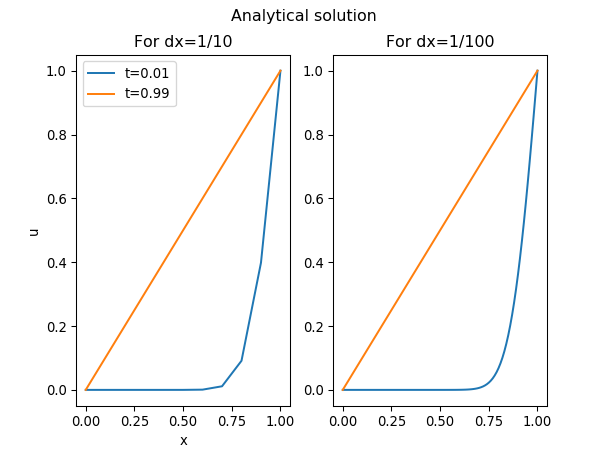
\includegraphics[width=140mm]{b.png}
	\caption{Analytical solution for $\Delta x = 1/10$ and $\Delta x =1/100$.}
	\label{fig:b}
\end{figure}

\begin{figure}[H]
	\centering
	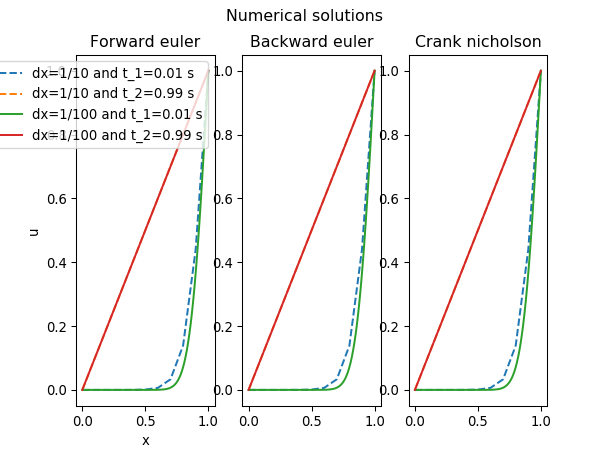
\includegraphics[width=140mm]{c.png}
	\caption{The numerical solution given different times $t_1$ and $t_2$ and spatial steps $\Delta x =1/10$ and $\Delta x = 1/100$.}
	\label{fig:c}
\end{figure}

\begin{figure}[H]
	\centering
	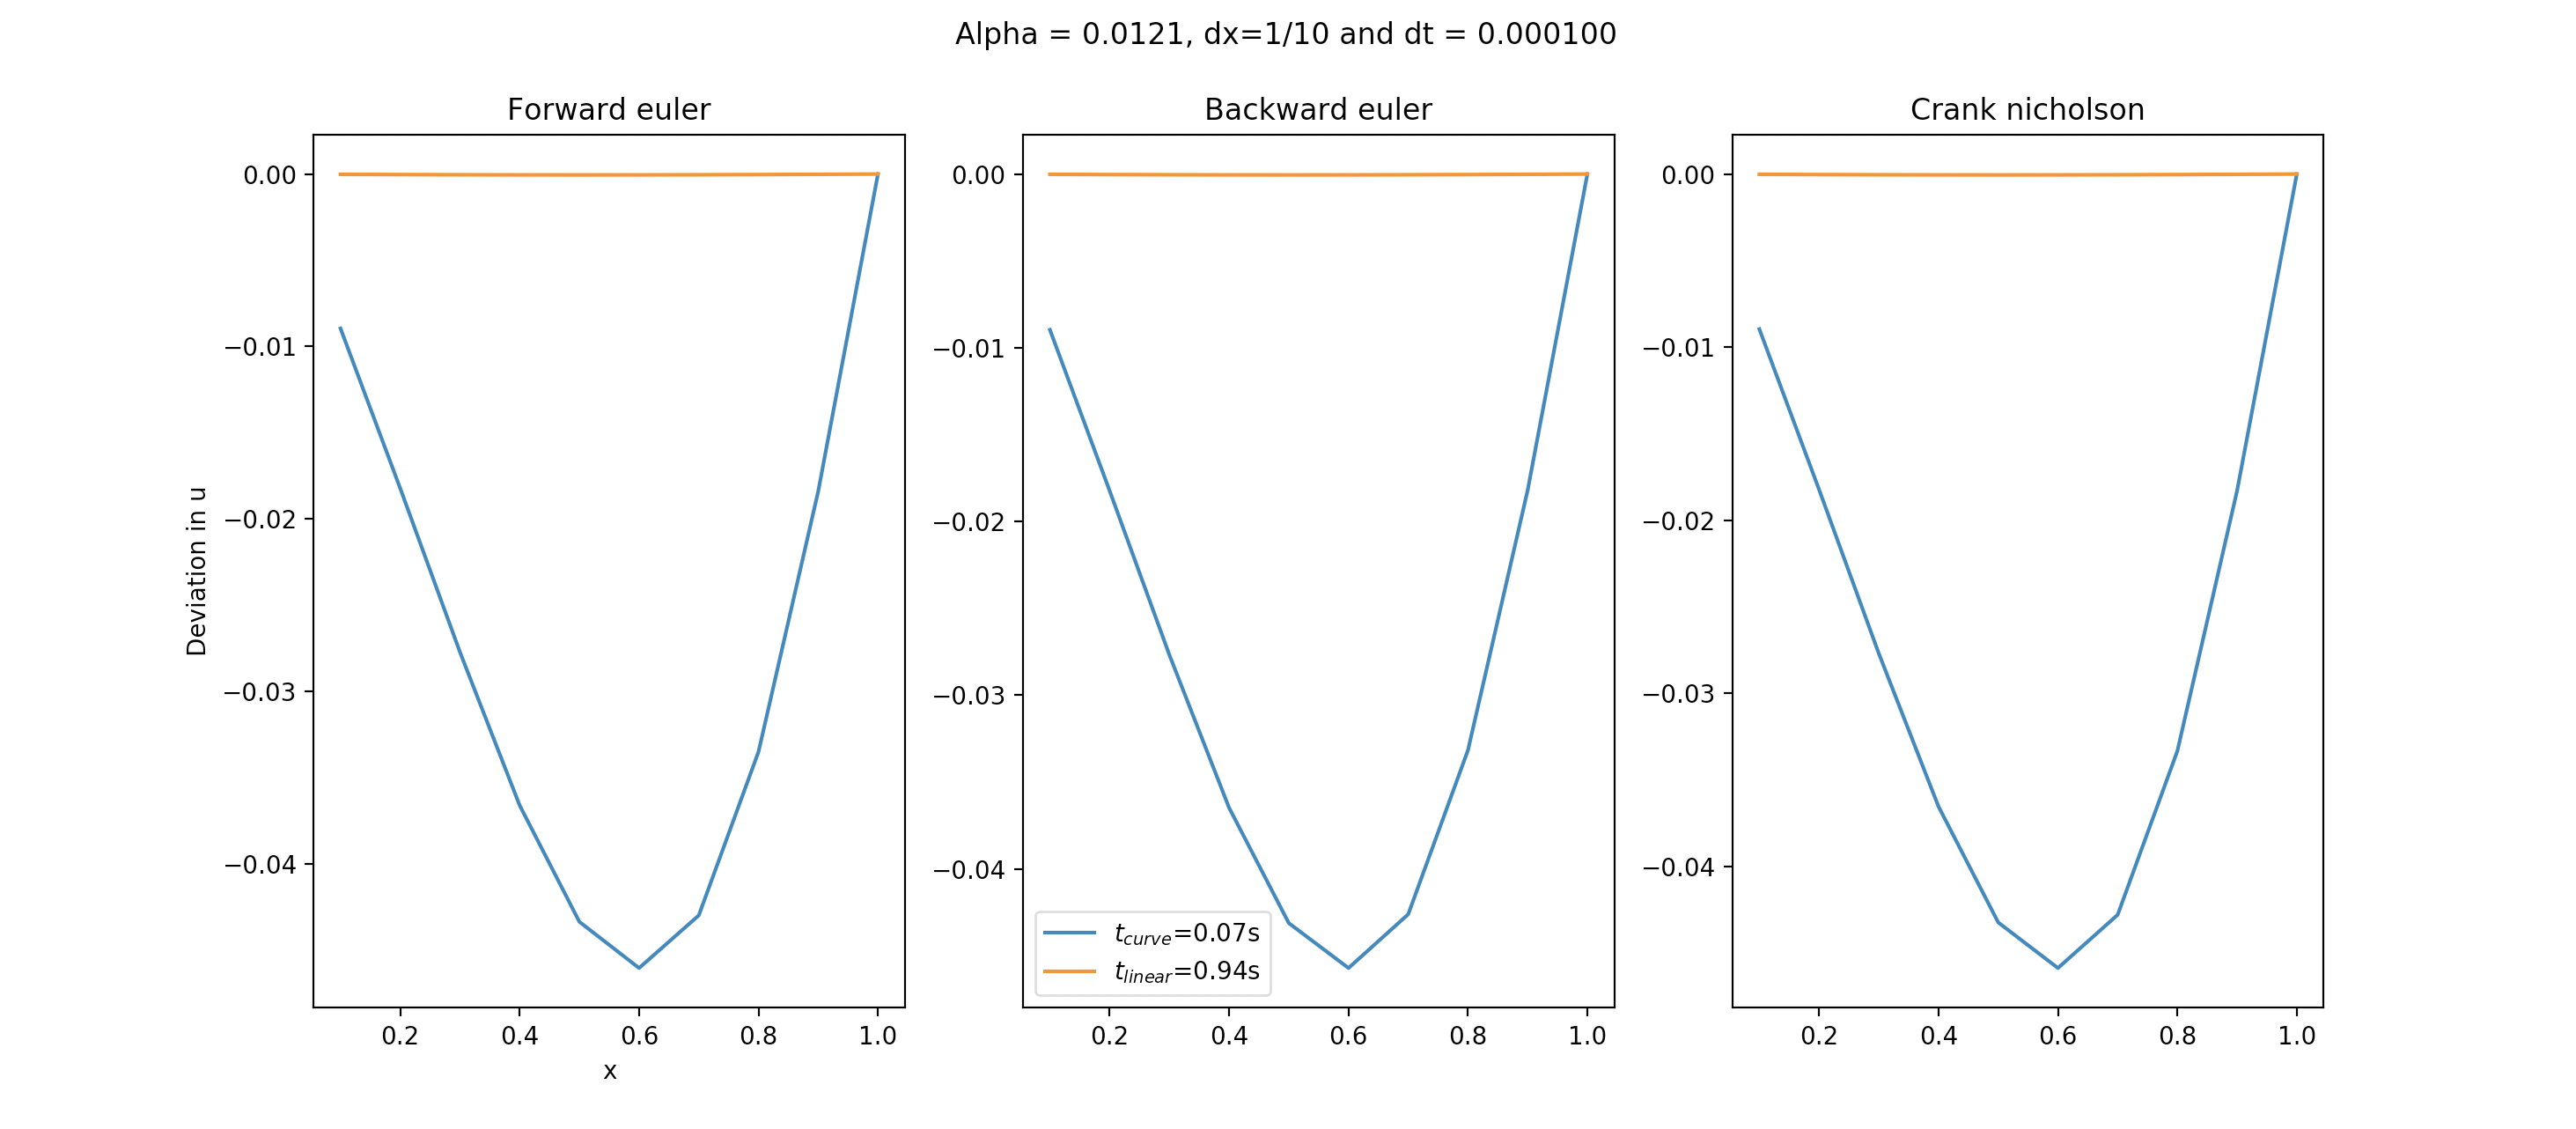
\includegraphics[width=180mm]{1_10}
	\caption{Deviation from analytical solution for $\alpha=0.0121$, $\Delta x=1/10$ and $\Delta t =0.0001$. The blue line $t_{curve}=0.07$ is the error after a short time period, where the solution is curved. The orange line $t_{linear}=0.94$ is the error after a longer time period, where the solution is linear.}
	\label{fig:1_10}
\end{figure}

\begin{figure}[H]
	\centering
	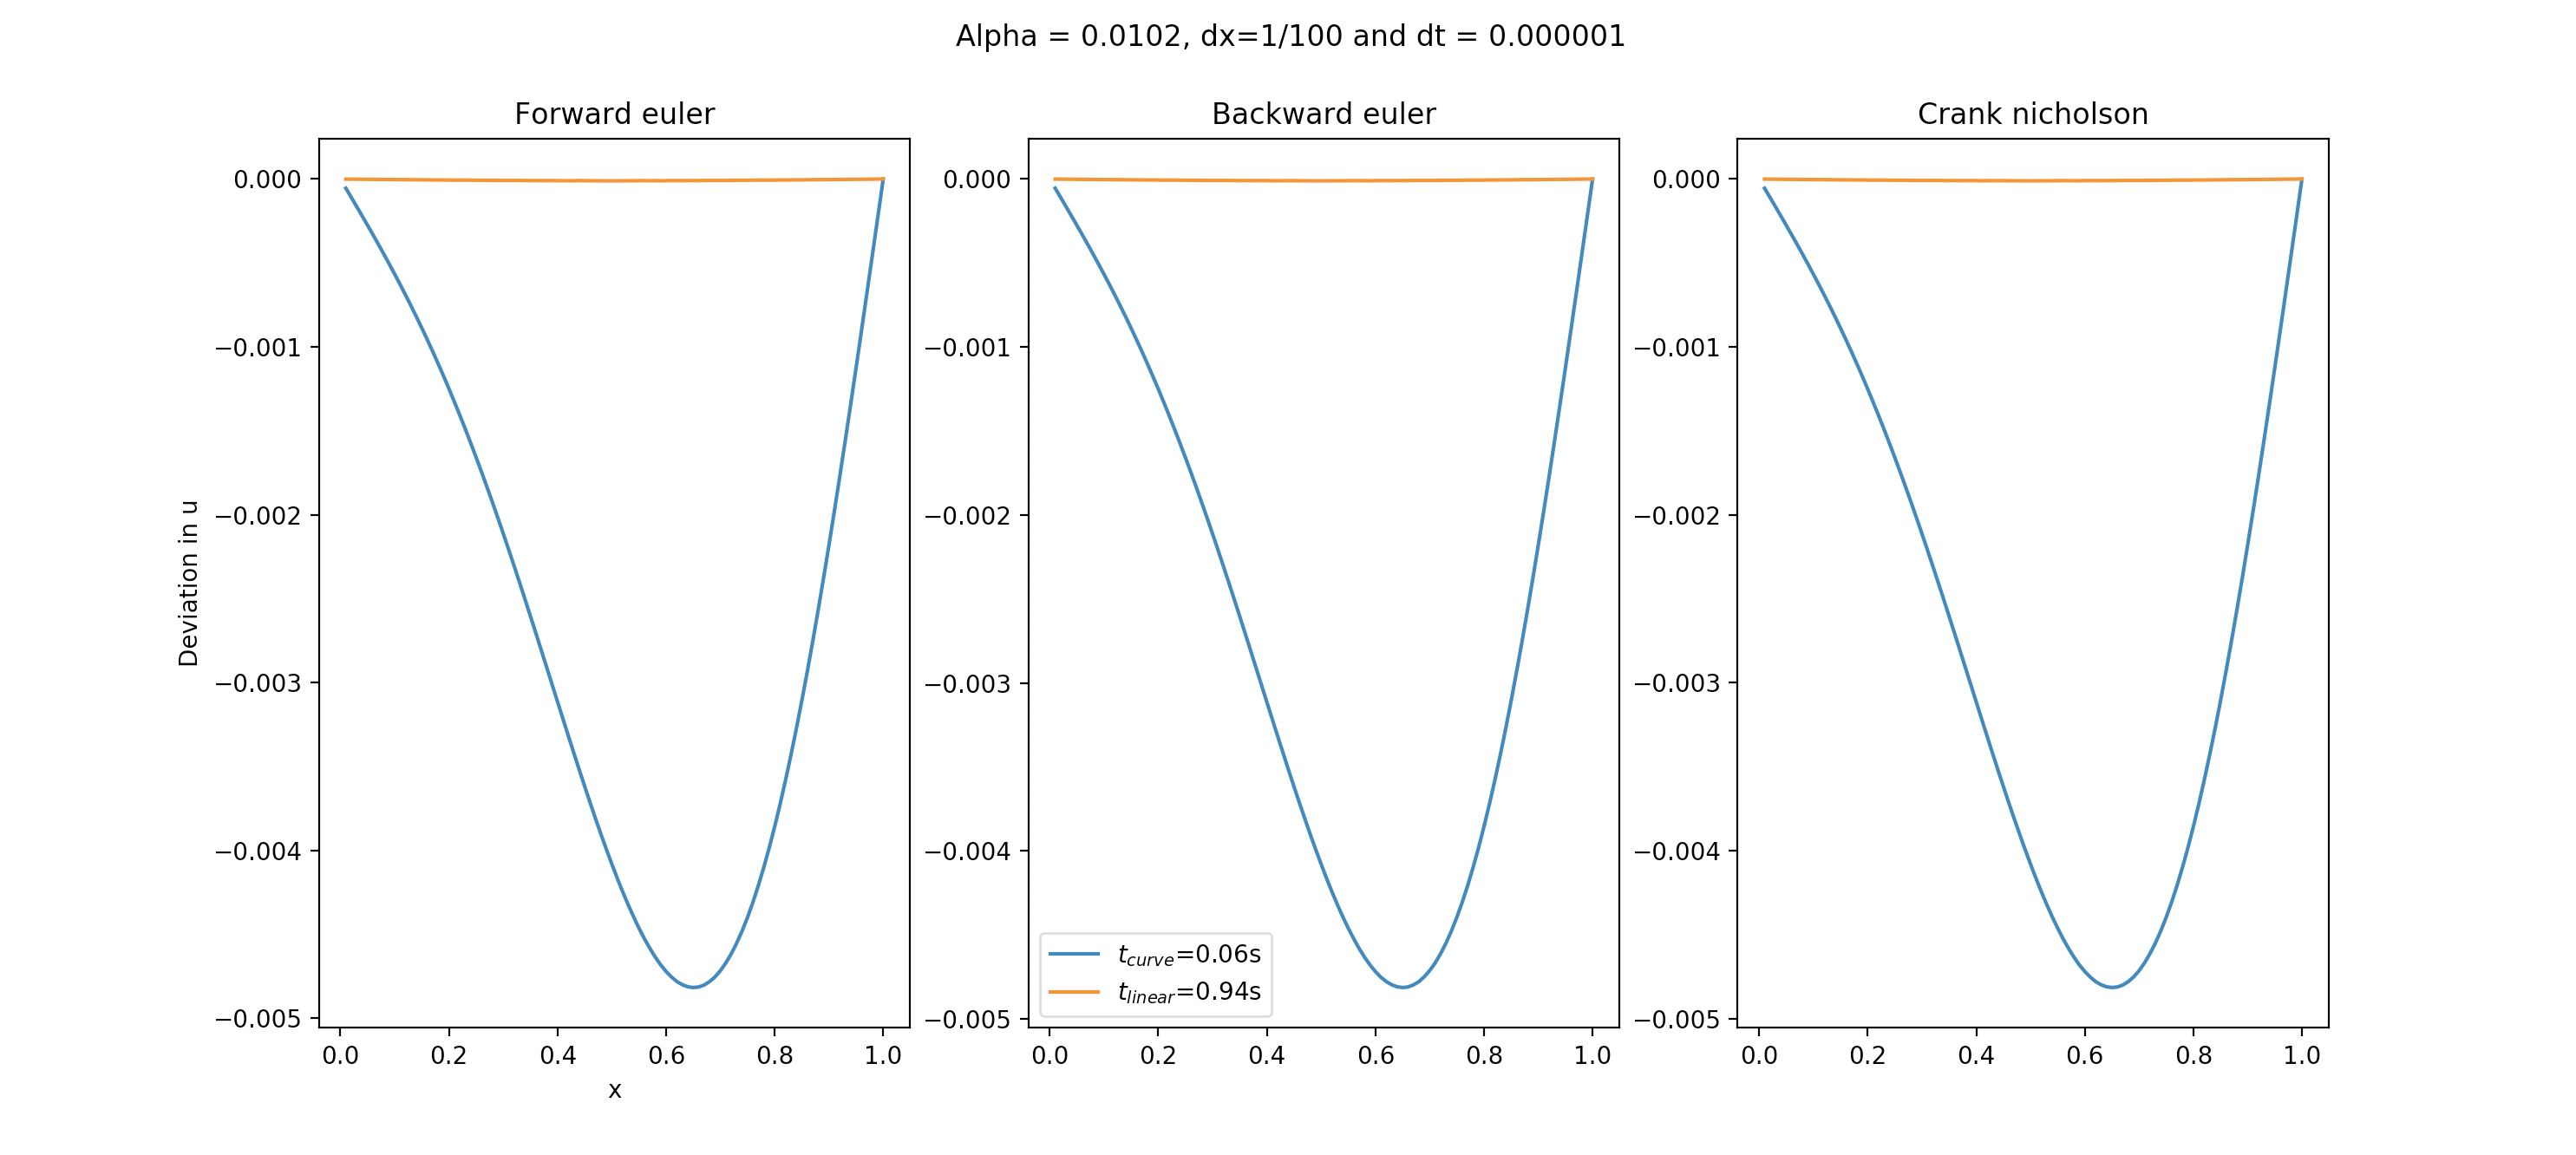
\includegraphics[width=180mm]{1_100}
	\caption{Deviation from analytical solution for $\alpha=0.0102$, $\Delta x=1/100$ and $\Delta t =0.000001$. The blue line $t_{curve}=0.06$ is the error after a short time period, where the solution is curved. The orange line $t_{linear}=0.94$ is the error after a longer time period, where the solution is linear.}
	\label{fig:1_100}
\end{figure}

\begin{figure}[H]
	\centering
	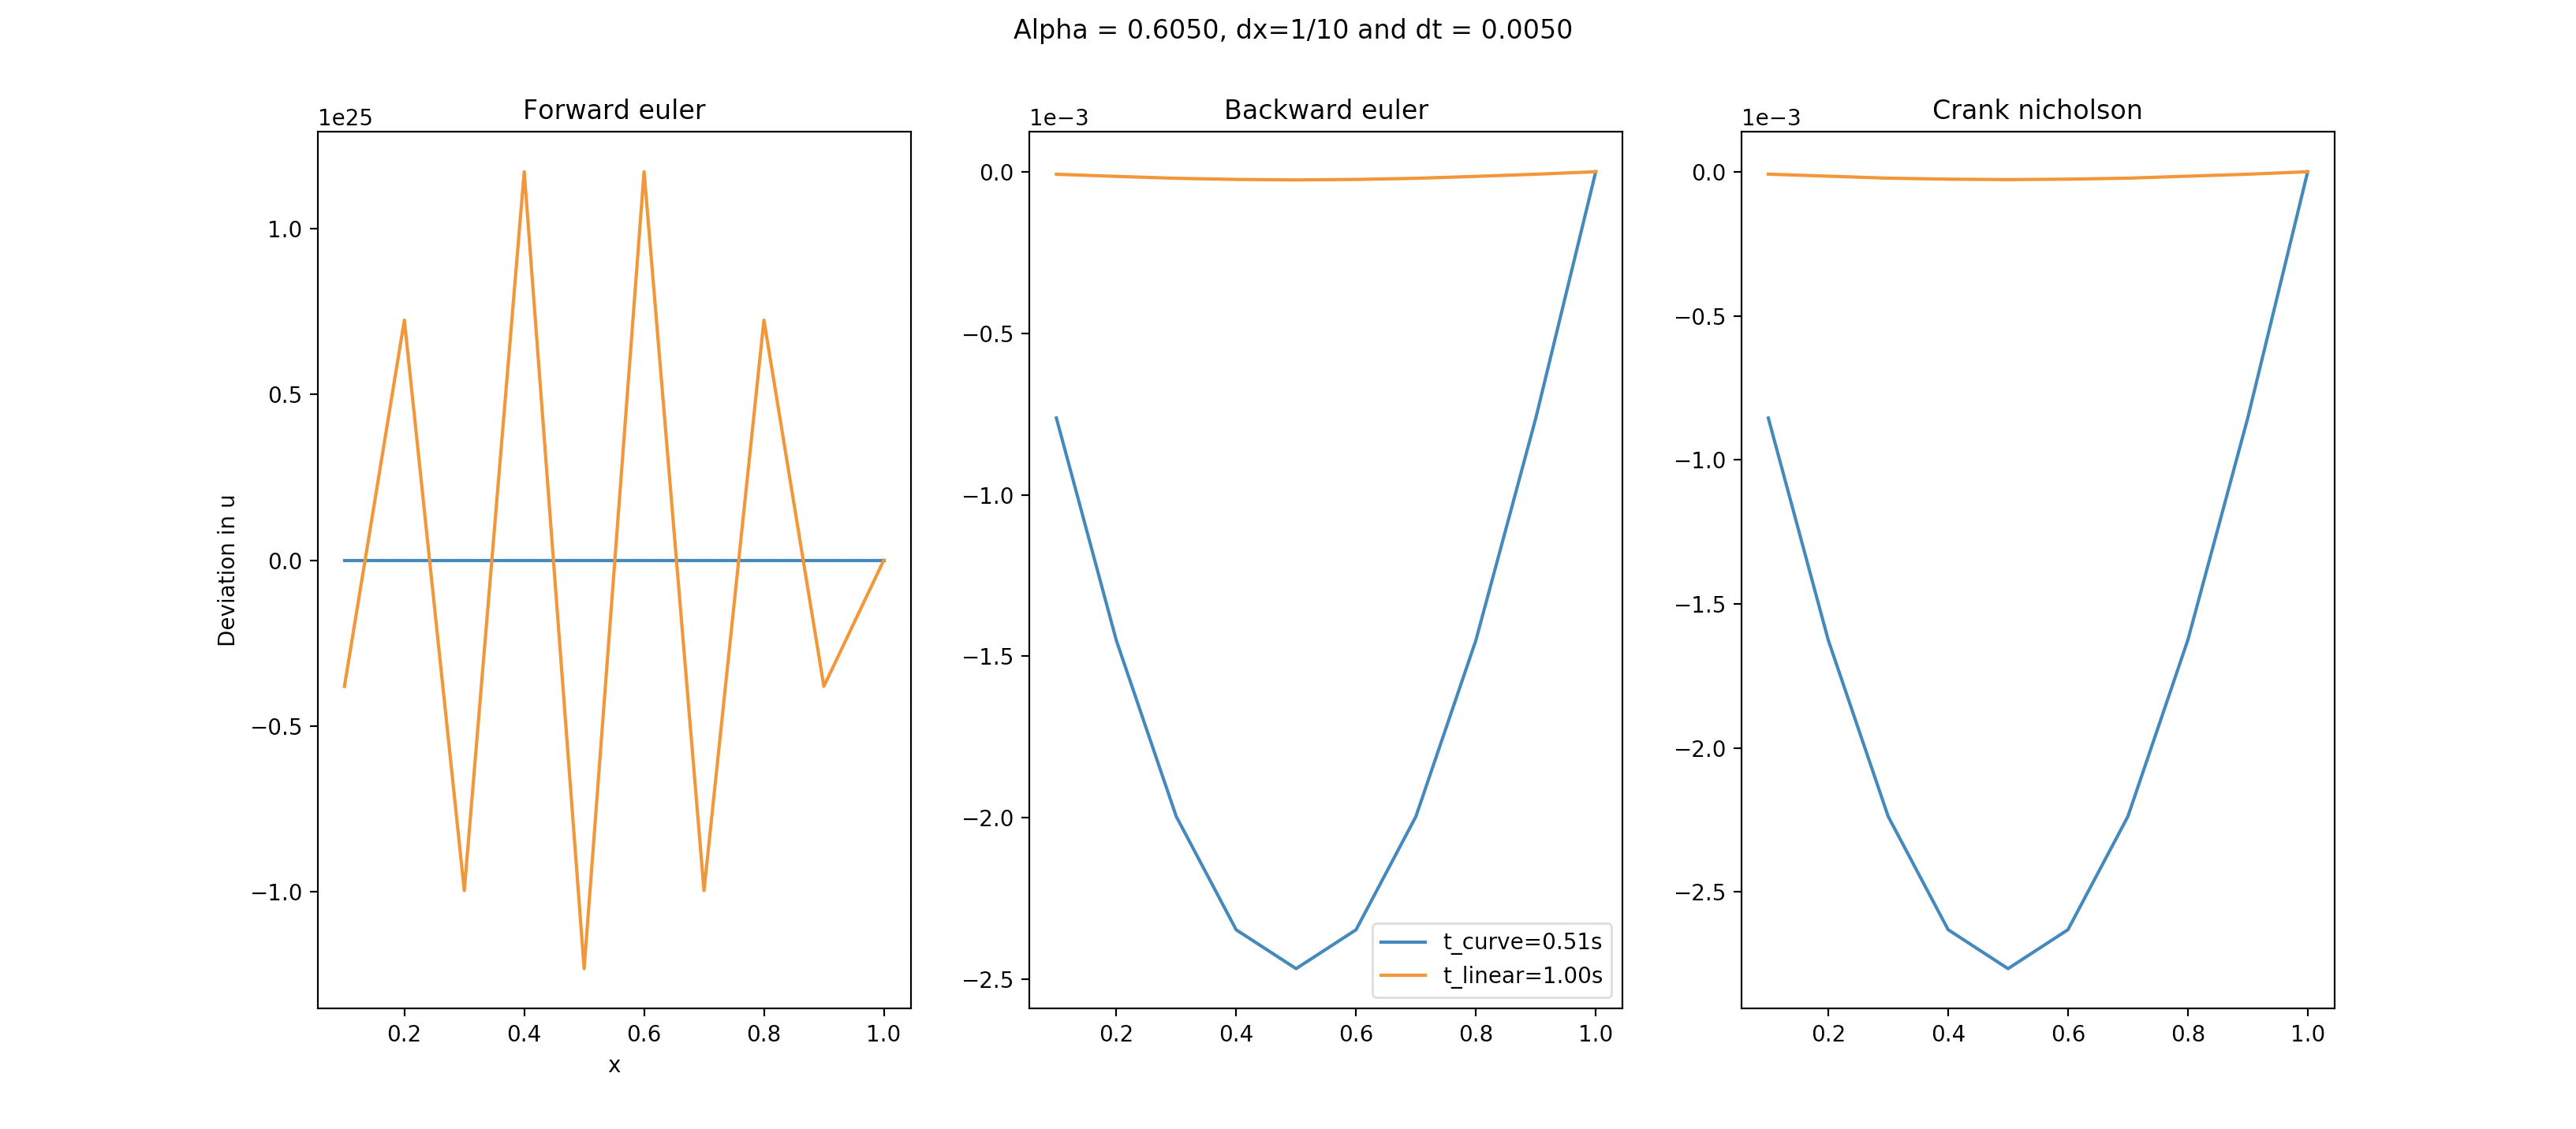
\includegraphics[width=180mm]{1_10_a}
	\caption{Deviation from analytical solution for $\alpha=0.6050$, $\Delta x=1/10$ and $\Delta t =0.005$. The blue line $t_{curve}=0.51$ is the error after a short time period, where the solution is curved. The orange line $t_{linear}=1.0$ is the error after a longer time period, where the solution is linear.}
	\label{fig:1_10_a}
\end{figure}

\begin{figure}[H]
	\centering
	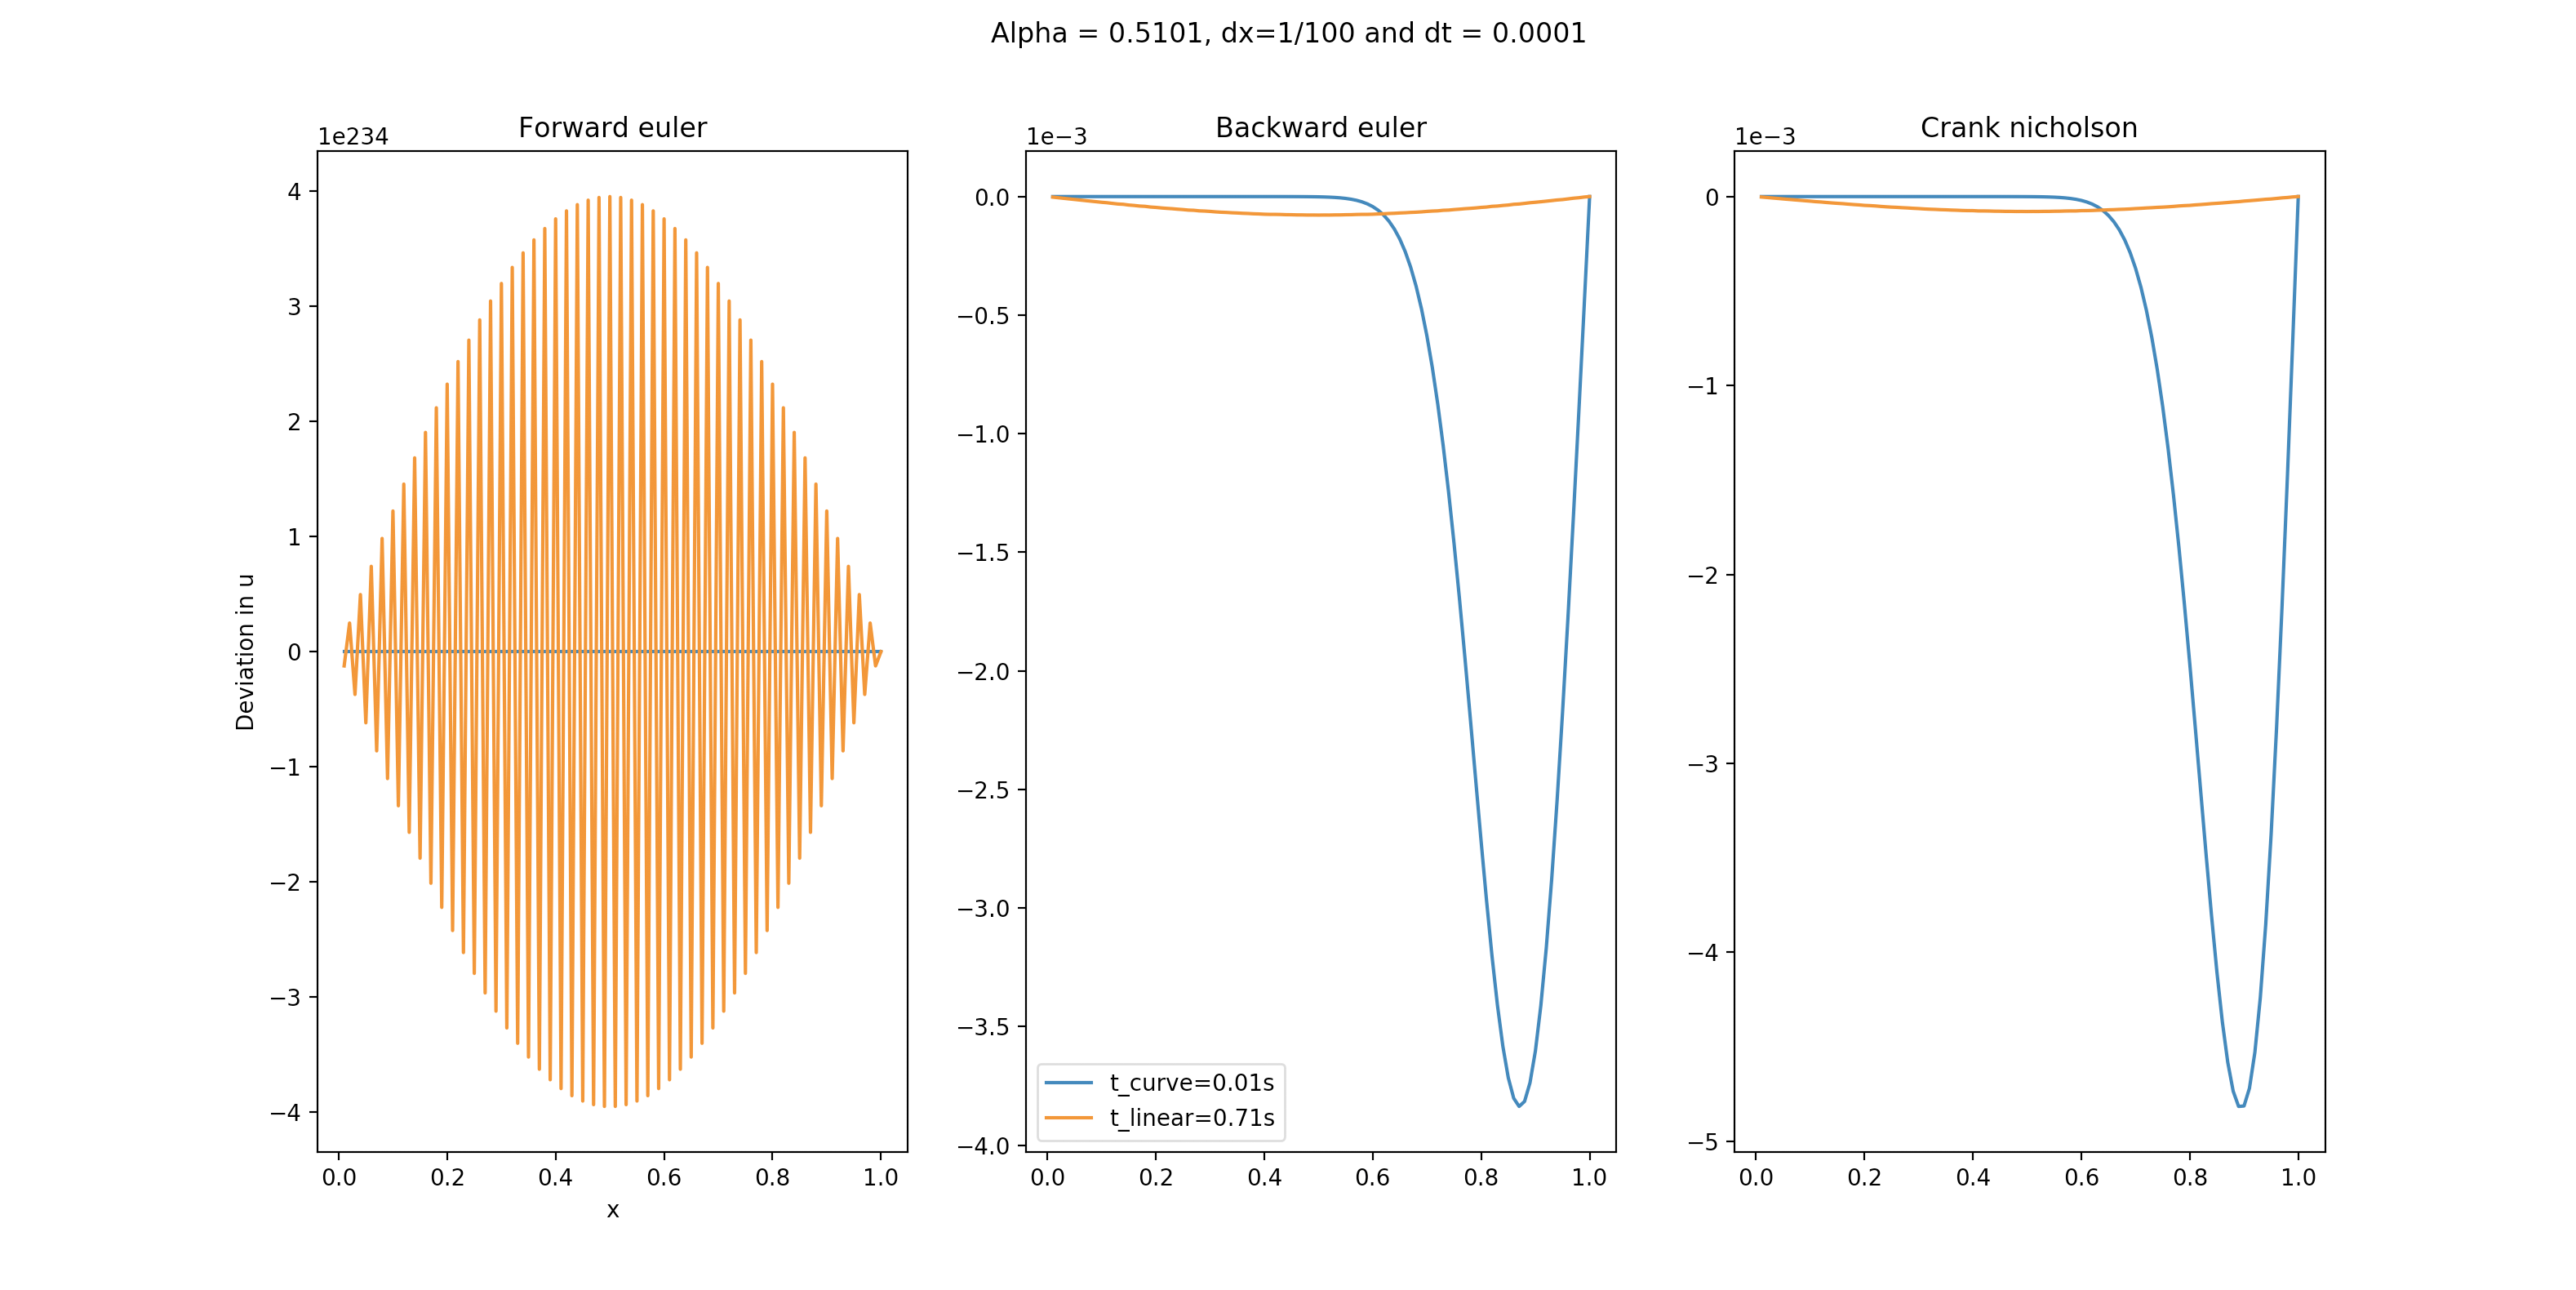
\includegraphics[width=180mm]{1_100_a}
	\caption{Deviation from analytical solution for $\alpha=0.5101$, $\Delta x=1/100$ and $\Delta t =0.0001$. The blue line $t_{curve}=0.01$ is the error after a short time period, where the solution is curved. The orange line $t_{linear}=0.71$ is the error after a longer time period, where the solution is linear.}
	\label{fig:1_100_a}
\end{figure}

\begin{figure}[H]
	\centering
	\includegraphics[width=120mm]{contour_0.png}
	\caption{Contour plot showing the temperature distribution for the beginning of 2D the simulation at $t=0$}
	\label{fig:contour0}
\end{figure}

\begin{figure}[H]
	\centering
	\includegraphics[width=120mm]{contour_1.png}
	\caption{Contour plot showing the temperature distribution for 2D simulation at $t=0.01$}
	\label{fig:contour1}
\end{figure}

\begin{figure}[H]
	\centering
	\includegraphics[width=120mm]{contour_2.png}
	\caption{Contour plot showing the temperature distribution for 2D simulation at $t=0.4$}
	\label{fig:contour2}
\end{figure}

\begin{figure}[H]
	\centering
	\includegraphics[width=140mm]{contour_plot.png}
	\caption{3D contour plot showing the temperature distribution for the lithosphere simulation as function of time passed and depth.}
	\label{fig:contour_3d}
\end{figure}

\begin{figure}[H]
	\centering
	\includegraphics[width=140mm]{T_vs_depth.png}
	\caption{Plot showing the temperature distribution for the lithosphere simulation as function of depth for different times.}
	\label{fig:T_vs_depth}
\end{figure}

\begin{figure}[H]
	\centering
	\includegraphics[width=140mm]{T_90km_vs_t_V2.png}
	\caption{Plot showing the temperature distribution for the lithosphere simulation as function of time for different depths.}
	\label{fig:T_90_vs_t}
\end{figure}

\subsection{Tables}


\begin{table}[H]
\begin{center}
\caption{Theoretical truncation errors.}
\begin{tabular}{  |c|c|c|c|c|c| } \hline
Scheme:&	Truncation error&Stability requirments \\ \hline
Crank Nicholson&$O(\Delta x^2) \text{ and } O(\Delta t^2)$&Stable for all\\ \hline
Backward Euler&$O(\Delta x^2)  \text{ and } O(\Delta t)$&Stable for all\\ \hline
Froward Euler&$O(\Delta x^2)  \text{ and } O(\Delta t)$&$\Delta t \leq 1/2\Delta x^2$\\ \hline
\end{tabular}
\label{tab:a}
\end{center}
\end{table}

\begin{table}[H]
\begin{center}
\caption{Simulation time for algorithms (1D case).}
\begin{tabular}{  |c|c|c|c|c|c| } \hline
Scheme:&	$\Delta x = 1/10$&$\Delta x = 1/100$ \\ \hline
Crank Nicholson&0.019732s&14.9372s\\ \hline
Backward Euler&0.021026s&14.5824s\\ \hline
Froward Euler&	0.00865s&3.58414s\\ \hline
\end{tabular}
\label{tab:time}
\end{center}
\end{table}

\begin{table}[H]
\begin{center}
\caption{RRMSE for the different algorithms for $t_1=0.01$.}
\begin{tabular}{  |c|c|c|c|c|c| } \hline
Scheme:&	$\Delta x =1/10$&$\Delta x = 1/100$ \\ \hline
Crank Nicholson&0.034560&0.0038095\\ \hline
Backward Euler&0.034521&0.0038079\\ \hline
Froward Euler&0.034599&0.0038086\\ \hline
\end{tabular}
\label{tab:error}
\end{center}
\end{table}

\begin{table}[H]
\begin{center}
\caption{RRMSE for the different algorithms for $t_2=0.99$.}
\begin{tabular}{  |c|c|c|c|c|c| } \hline
Scheme:&	$\Delta x =1/10$&$\Delta x = 1/100$ \\ \hline
Crank Nicholson&$9.5847294\times 10^{-5}$&$6.7524668\times10^{-5}$\\ \hline
Backward Euler&$9.5847294\times 10^{-5}$&$6.7524668\times10^{-5}$\\ \hline
Froward Euler&$9.5847294\times 10^{-5}$&$6.7524668\times10^{-5}$\\ \hline
\end{tabular}
\label{tab:error2}
\end{center}
\end{table}

\clearpage

\section{Appendix}

\subsection{General algorithm for tri-diagonal matrix}

There exists an algorithm for solving generic sets of linear equations, but in the case for implicit methods where we have a tri-diagonal matrix we can use a different algorithm which decreases the amount of floating point operations needed. We denote the elements in the leading diagonal of A as $b_1, b_2, ..., b_n$, the elements above the leading diagonal as $a_2, a_3 ..., a_n$, and the elements below the leading diagonal as $c_1, c_2, ..., c_{n-1}$. The algorithm uses a forward substitution to replace the leading diagonal with elements denoted by $\tilde{b}_i$, and replaces the righthand side in with the elements $\tilde{f}_i$ as shown below\cite{98}:
\begin{align*}
\tilde{b}_i=b_i-\frac{a_ic_{i-1}}{\tilde{b}_{i-1}} \\
\tilde{f}_i=f_i-\frac{a_i\tilde{f}_{i-1}}{\tilde{b}_{i-1}}
\end{align*}
where $\tilde{b}_1=b_1$ and $\tilde{f}_i=f_i$. The algorithm then continues with a backward substitution which gives the solution:
\begin{align}
u_{i-1}=\frac{\tilde{f}_{i-1}-c_{i-1}u_i}{\tilde{b}_{i-1}}
\end{align}
\\

\subsection{Analytical expression for 1D diffusion equation}

The one dimensional diffusion equation has an analytical expression for the continuous problem. 

\begin{equation}
\nabla ^2 u(x,t)=\frac{\partial u(x,t)}{\partial t}
\label{eq:a1d}
\end{equation}

The initial condition is $u(x,0)=g(x)$, when $0<x<L$. We also have $u(0,t)=0$ and $u(L,t)=0$, when $t\leq0$. We use separation of variables when solving \ref{eq:a1d}:

\begin{equation}
u(x,t) = F(x)G(t)
\label{eq:sep}
\end{equation}

This gives us one function only depending on position x and one only depending on time t. We get the set of equations:

\begin{equation*}
\frac{\partial u}{\partial t} = F \frac{\partial G}{\partial t}
\end{equation*}

and

\begin{equation*}
\frac{\partial^2 u}{\partial x^2} = G \frac{\partial^2 F}{\partial x^2}
\end{equation*}

We can now use the relation given equation \ref{eq:heat_one}:

\begin{equation}
\begin{split}
&F\frac{\partial G}{\partial t} = G \frac{\partial ^2 F}{\partial x^2}\\
&\frac{1}{G}\frac{\partial G}{\partial t} = \frac{1}{F} \frac{\partial^2 F}{\partial x^2}
\end{split}
\end{equation}

We set the equations equal to a negative constant $-\lambda^2$. This gives us the solutions:

\begin{equation*}
\begin{split}
G &= Ae^{-\lambda^2 t}\\
F &= B\cos{(\lambda x)} + C\sin{(\lambda x)}
\end{split}
\end{equation*} 

We can now use equation \ref{eq:sep} to find the general solution u:

\begin{equation}
\begin{split}
u &= GF = Ae^{-\lambda^2 t} [B\cos{(\lambda x)} + C\sin{(\lambda x)}]\\
&=e^{-\lambda^2 t} [C_1\cos{(\lambda x)} + C_2\sin{(\lambda x)}]
\end{split}
\end{equation}

The boundary conditions gives us the solution:

\begin{equation}
u(x,t) = A_n\sin{(n\pi x/L)}e^{-n^2\pi^2t/L}
\end{equation}

We have infinitely many solutions to this equation, due to the n factor. We can use a superposition of these solutions since the diffusion equation is linear:

\begin{equation}
u(x,t) = \sum_{n=1}^{\infty}A_n\sin{(n\pi x/L)}e^{-n^2\pi^2t/L}
\label{eq:u_undfA}
\end{equation}

We decide the coefficient $A_n$ by using the initial condition:

\begin{equation}
u(x,0)=g(x)=\sum_{n=1}^{\infty}A_n\sin{(n\pi x/L)}
\end{equation}

Which gives us that:

\begin{equation*}
A_n=\frac{2}{L}\int_0^Lg(x)\sin{(n\pi x/L)} dx
\end{equation*}

We need to find the function g(x). We should obtain an equilibrium temperature when the time goes to infinity. This can be written as:

\begin{equation*}
\lim_{t \to \infty} u(x,t) = u_E(x)
\end{equation*}

Where $u_E(x)$ is the equilibrium temperature. We can look at how this function behaves given the boundary conditions:

\begin{equation*}
\frac{d^2 u_E}{dx^2}=0 \hspace{0.5cm} u_E(0)=0\hspace{0.5cm} u_E(L)=1
\end{equation*}

This gives us the general solution:

\begin{equation*}
u_E(x)=k_1x + k_2
\end{equation*}

Where $k_1$ and $k_2$ are constants. We get the function $u_E(x)=x/L$. Now we define a new function $v(x,t)=u(x,t)-u_E(x)$, where $u(x,t)$ is the solution to equation \ref{eq:u_undfA}, which we wish to solve for:

\begin{equation}
u(x,t)=v(x,t)+u_E(x)
\label{eq:vu}
\end{equation}

We need to know the boundary and initial conditions for $v(x,t)$:

\begin{equation*}
\begin{split}
&v(x,0)=u(x,0)-u_E(x)=0-x/L=-x/L\\
&v(0,t)=u(0,t)-u_E(0)=0-0=0\\
&v(L,t)=u(L,t)-u_E(L)=1-1=0
\end{split}
\end{equation*}
 
 We use the same method as earlier and find the solution for v(x,t):
 
 \begin{equation}
v(x,t) = \sum_{n=1}^{\infty}B_n\sin{(n\pi x/L)}e^{-n^2\pi^2t/L}
\end{equation}
 
Where the coefficient $B_n$ is given by:

\begin{equation}
B_n=\frac{2}{L}\int_0^Lg(x)\sin{(n\pi x/L)} dx
\end{equation}

Now we can use the fact that g(x)=v(x,0)=-x/L and equation \ref{eq:vu}:

\begin{equation}
u(x,t)=x/L+\sum_{n=1}^{\infty}\frac{2}{L}\int_0^L(-x/L)\sin{(n\pi x/L)} dx\sin{(n\pi x/L)}e^{-n^2\pi^2t/L}
\end{equation}

We solve the integral and find the final solution:

\begin{equation*}
\begin{split}
&\int_0^L(-x/L)\sin{(n\pi x/L)} dx=\frac{L(\pi n \cos{(\pi n)}-\sin{(\pi n)})}{\pi^2n^2}\\
&\Rightarrow u(x,t)=x/L+\sum_{n=1}^{\infty}\frac{2(\pi n \cos{(\pi n)}-\sin{(\pi n)})}{\pi^2n^2}\sin{(n\pi x/L)}e^{-n^2\pi^2t/L}
\end{split}
\end{equation*}

We now have a analytical expression for heat diffusion in one dimension \cite{94}\cite{96}. 

\clearpage

\begin{thebibliography}{9}
\bibitem{94}
	Jensen, M.H., 2015, Computational Physics Lecture Notes Fall 2015
\bibitem{95}
	Jensen, M.H., 2017, Computational Physics Lectures: Statistical physics and the Ising Model
\bibitem{96}
	Dawkins, Paul., 2018, Heat Equation With Non-Zero Temperature Boundaries
\bibitem{97}
	Despotovic, M, et al., 2016, Evaluation of empirical models for predicting monthly mean horizontal diffuse solar radiation
\bibitem{98}
	Amundsen, S, et al., 2020, Project 1
	
\end{thebibliography}

\end{document}